% concatenated from Valuatively_Independent_Bases_For_Fermat_Family_of_Cubic_Curves.tex
\documentclass{article}
\usepackage{amsfonts,amsmath,amssymb,amsthm}
\usepackage{tikz}
\usepackage{graphicx} % Required for inserting images
\usepackage{geometry}
\geometry{margin=2.5cm}
\newcommand{\PP}{\mathbb{P}}
\newcommand{\QQ}{\mathbb{Q}}
\newcommand{\CC}{\mathbb{C}}
\newcommand{\RR}{\mathbb{R}}
\newcommand{\ZZ}{\mathbb{Z}}
\newcommand{\op}[1]{\operatorname{#1}}
\newcommand{\Star}{\operatorname{Star}}
\newcommand{\conv}{\operatorname{conv}}
\newcommand{\val}{\operatorname{val}}
\newcommand{\supp}{\operatorname{supp}}

\newtheorem{theorem}{Theorem}
\newtheorem{conj}{Conjecture}
\newtheorem{prop}{Proposition}
\newtheorem{lemma}{Lemma}
\newtheorem{rem}{Remark}
\newtheorem{corollary}{Corollary}
\newtheorem{definition}{Definition}
\newtheorem{remark}{Remark}

\title{Valuatively independent bases for the Fermat family of cubic curves}

\author{Jakob Hultgren and Sohaib Khalid}
\begin{document}

\maketitle

\begin{abstract}
    Let $\pi:(X,L)\rightarrow \mathbb D^*$ be the Fermat family of cubic curves in $\mathbb P^2$. For each $k\geq 1$, we construct a valuatively independent basis for $H^0(X,L^k)$. The construction uses a canonical cost function determined by a Hessian structure on the essential skeleton $\op{Sk}(X,\pi)$.
\end{abstract}

\section{Introduction}
Given a polarised degenerating family $\pi:(X,L) \to \mathbb D^*$ of Calabi-Yau manifolds which is meromorphic over the punctured unit disc $\mathbb D^*$, a central problem in complex geometry is to determine the limiting behaviour of the canonical Ricci-flat \emph{Calabi-Yau} metrics $\omega_t\in c_1(L_t)$ on the fibres $X_t$ as $t\to 0$. A very important special case is when the degeneration is a \emph{large complex structure limit point}, which is the subject of the \emph{Strominger--Yau--Zaslow (SYZ)} picture of mirror symmetry. A key expectation in this picture is the \emph{metric SYZ conjecture}, which states that, given any $\delta>0$, there should exist $\varepsilon > 0$ such that whenever $0< |t|<\varepsilon$, the fibre $X_t$ admits an open subset 
$U_t\subseteq X$ whose Calabi-Yau volume satisfies $|U_t|\geq (1-\delta)|X_t|$
%\[
%\int_{U_t}\omega_t^{\dim_\CC X_t} \geq (1-%\delta)\int_{X_t}\omega_t^{\dim_\CC X_t}
%\]
and which admits a smooth map $U_t\to B$ whose fibres are special Lagrangian tori of $(X_t,\omega_t)$. 

A program initiated by Yang Li uses techniques from non-Archimedean geometry together with local and global stability estimates for real and complex Monge-Ampère equations to prove this, and under this program, the metric SYZ conjecture has been verified in several cases \cite{LiFermat,PS,HJMM,LiToric,AH}. The main obstacle in carrying out this program in full generality is producing solutions to certain real Monge-Ampère equations. Crucially, \cite{LiNA} shows that the metric SYZ conjecture holds for $\pi:X\to \mathbb D^*$ if the solution to the non-Archimedean Monge-Ampère equation simultaneously solves a real Monge-Ampère equation, in an appropriate sense. 

Due to the close connections between the theory of real Monge-Ampère equations and the theory of optimal transport, it is  natural to attempt to formulate an optimal transport problem whose optimiser can be shown to solve both the non-Archimedean and the real Monge-Ampère equation. This is indeed the approach taken in \cite{HJMM,LiToric,AH}. More generally, the picture that emerges from this is that such an optimal transport problem should be formulated on $\operatorname{Sk}(X,\pi)\times B$ where $B$ is to be thought of as the essential skeleton  $\operatorname{Sk}(X^\vee,\pi^\vee)$ of a degenerating family $\pi^\vee:X^\vee\to \mathbb D^*$ mirror to $\pi:X\to\mathbb D^*$. In \cite{LiCanonicalBasis}, Yang Li has proposed a conjectural picture where canonical bases of $H^0(X,L^k), k\geq 1$ are identified with lattice points in the top-dimensional faces of $B$ and the correct cost function for the optimal transport problem appears as the limit of straightforward valuations in these basis elements 
\begin{equation}\label{eq:ValuativeCost} c_k(x,s) = k^{-1}\val_x(s), x\in \operatorname{Sk}(X^\vee,\pi^\vee), s\in H^0(X,L^k)\subset B. 
\end{equation}
By the main result in \cite{LiCanonicalBasis}, the resulting optimal transport problem would produce the solution to the non-Archimedean Monge-Ampère equation if the canonical bases satisfy the property of \emph{valuative independence} (see Section~\ref{sec:Bases}) globally on $\op{Sk}(X,\pi)$.  However, showing existence of such bases seems like a challenging problem. 

The purpose of this note is to provide an explicit construction of a sequence of bases $H^0(X,L^k), k\geq 1$ when $(X,L)$ is given by the Fermat family of cubic curves in $\mathbb P^2$. 
\begin{theorem}\label{thm:main}
    Let $X$ be the Fermat family of curves in $\mathbb P^2$ 
    $$ xyz-t(x^3+y^3+z^3) = 0, $$
    polarized by the restriction $L$ of $-K_{\mathbb P^2}$ and let $k\geq 1$. Then $H^0(X,L^k)$ has a valuatively independent basis.
\end{theorem}
%Here, the natural candidate for $B$ is given by the boundary of the moment polytope of $\mathbb P^2$ and monomial sections of $H^0(X,L^k), k\geq 1$, are naturally identified with its lattice points. The theorem is proved inductively, constructing a valuatively independent basis for  sequence of bases inductively in the level $k$, using explicit linear combinations of monomials and basis elements at lower levels. %To the best of the authors' knowledge, no such construction seems to have been previously known. 

In Theorem~\ref{thm:main}, the natural candidate for $B$ is given by the boundary of the (anti-canonical) moment polytope of $\mathbb P^2$ and monomial sections of $H^0(X,L^k), k\geq 1$, are naturally identified with its lattice points. Moreover, $\op{Sk}(X,\pi)$ carries a natural Hessian structure induced by the toric data of $\mathbb P^2$ (see Section~\ref{sec:CostFunction}). 
We recall that a basis $\theta_1,\ldots,\theta_r$ of $H^0(X,L^k)$ is valuatively independent if for any $n\in \op{SK}(X,\pi)$ and functions rational functions $a_i$, 
\begin{equation}
val_n((a_1\theta_1+\dots+a_r\theta_r)/\tau) = \min\{val_t(a_i)+val_n(\theta_i/\tau) \ : \ a_i \neq 0 \}. \label{eq:ValIndep}
\end{equation}
%Equivalently (in the case of curves), each section $\theta_l$ has a unique leading term (in terms of $n\in \op{SK}(X,\pi)$). 
As explained in \cite{LiCanonicalBasis}, constructing a basis which is \emph{locally} valuatively independent, i.e. satisfies \eqref{eq:ValIndep} for all $n$ in a small open set of $\op{Sk}(X,\pi)$, is a relatively straightforward task. The key difficulty is to produce a basis such that \eqref{eq:ValIndep} holds globally on $\op{Sk}(X,\pi)$. A central idea in our method of proof is to use a canonical cost function $c:\op{Sk}(X,\pi)\times B \to \RR$ induced by the Hessian structure on $\operatorname{Sk}(X^\vee,\pi^\vee)$, and look for a basis satisfying~\eqref{eq:ValuativeCost}. The canonical cost function $c$, which was introduced in \cite{HO}, is explicitly computable using the monodromy data of $\op{Sk}(X,\pi)$ as an affine manifold (see Section~\ref{sec:CostFunction}). Combined with the ansatz \eqref{eq:ValuativeCost} proposed in \cite{LiCanonicalBasis}, it provides, for each basis element, an \emph{a priori} indication of the vanishing orders along each strata of the central fiber, and thus a heuristic for how to construct such a global basis. From the explicit expression for $c$, we can inductively construct the valuatively independent basis for $H^0(X,L^k)$ from valuatively independent bases for $H^0(X,rL)$ with $r<k$ by adding correction terms to monomials of the form $\lambda\sigma \cdot S$ where $\sigma$ is a section given by an appropriate monomial term, $S$ is an appropriate member of the valuatively independent basis of $H^0(X,rL)$ 
%with $r<k$ 
and $\lambda$ is an appropriate constant. 

%Theorem~\ref{thm:main} gives a proof of the following fact: 
%\begin{cor}
%\end{cor}

\section{Cost function in the theory of Hessian manifolds}\label{sec:CostFunction}
An affine $\mathbb R$-bundle $L$ over an affine manifold $M$ is a principal $(\mathbb R,+)$-bundle with affine transition functions. Equivalently, $L$ is an affine manifold equipped with an affine map $L\rightarrow M$ with fibers isomorphic to $\mathbb R$ admitting local trivializations $\{U_i\times \mathbb R,p_i)$ such that the transition functions $p_i\circ p_j^{-1}:(U_j\cap U_i)\times \mathbb R\rightarrow U_i\times \mathbb R$ are of the form 
$$ (n,y)\rightarrow (n,y+\alpha_{ij}(x)) $$
for some affine transition function $\alpha_{ij}:U_j\cap U_i\rightarrow \mathbb R$.

Indeed, the toric data $\Delta, \Delta^\vee$ of $\mathbb P^2$ determines an affine manifold equipped with an affine $\mathbb R$-bundle. To see this, we fix a choice of integral basis $e_1, e_2$ in $\RR^2$ such that 
\[\Delta = \op{conv}(-e_1-e_2, -e_1+2e_2,2e_1-e_2),\quad \Delta^\vee = \op{conv}(-e_1^\vee, e_1^\vee + e_2^\vee,-e_2^\vee). \]
For future reference, we denote
\[
m_0 = -e_1-e_2, m_1 = -e_1+2e_2, m_2 = 2e_1-e_2, \quad n_0 = -e_1^\vee, n_1 = e_1^\vee + e_2^\vee, n_2=-e_2^\vee.
\]

\begin{center}
    \begin{tikzpicture}
        \draw 
        (-1,-1) node[left] {$m_0$}
        -- 
        (-1,2) node[above] {$m_1$}
        -- 
        (2,-1) node[right] {$m_2$}
        -- 
        (-1,-1);
        \draw 
        (5,0) node[left] {$n_0$}
        -- 
        (7,1) node[right] {$n_1$}
        -- 
        (6,-1) node[below] {$n_2$}
        -- 
        (5,0);
    \end{tikzpicture}
\end{center}
Note also that we have labelled the $m_k$ and $n_\ell$ in such a way that for $k=0,1,2$, 
we have 
\[
\langle m_k,n_k \rangle = \langle m_{k+1}, n_k \rangle = \langle m_k, n_{k-1}\rangle = 1, \quad \langle m_k, n_{k+1} \rangle = -2,
\]
where we take the subscripts modulo 3. We denote by $\Pi$ the fundamental group $\pi_1(\partial \Delta^\vee,n_0)$, and identify it with $\ZZ$ by taking the clockwise generator $\gamma$ to be positive.

The dual intersection complex of the central fibre $\{x_0x_1x_2=0\}$ is naturally identified with $\partial \Delta^\vee$. This is an affine manifold in a natural way. One way to specify its affine structure is as follows. The map $\pi:\RR \to \partial \Delta^\vee$ given for $t\in[k,k+1)$ by 
\[
\pi(t) = (k+1-t)n_k + (t-k)n_{k+1}
\]
(where the subscripts are taken modulo 3) is a universal covering map, and its various local inverses give affine coordinates around each point of $\partial \Delta^\vee$. For example, a local inverse of $\pi$ is given by 
\[
\varphi_k: U_k \to (k-1,k+1), n\mapsto k + \frac{1}{3}\langle m_{k+1}-m_k,n\rangle.
\]
Here and henceforth in this section, $U_k$ denotes the (open) star of the vertex $n_k$ in $\partial \Delta^\vee$, for $k=0,1,2$. Note that we have made choices for the basepoints of the covering map in such a way that $\varphi_0(n) = \varphi_1(n)$, $\varphi_1(n) = \varphi_2(n)$ but $\varphi_2(n) = \varphi_0(n) + 3$ whenever both sides are defined.

Next, we describe the affine $\RR$-bundle $L$ on $M=\partial\Delta^\vee$ which admits convex sections. (This determines $M= \partial\Delta^\vee$ as a Hessian manifold.) Observe that the map $n\mapsto -\langle m_k,n\rangle$ is piecewise affine and convex on $U_k$. We directly verify this using affine coordinates furnished by (the local inverses of) $\pi$. Indeed, for $t\in (k-1,k)$, we have 
\[
-\langle m_k, \pi(t)\rangle = -\langle m_k, (k-t)n_{k-1}+(t-k+1)n_k\rangle = -1,
\]
and for $t\in [k,k+1)$, we have 
\[
-\langle m_k, \pi(t)\rangle = -\langle m_k, (k+1-t)n_{k}+(t-k)n_{k+1}\rangle = 3t-3k-1.
\]
This shows that on $U_k$, the map $n\mapsto -\langle m_k, n\rangle $ is given by 
\[n\mapsto \max\{-1,3\varphi_k(n)-3k-1\}\]
which is piecewise affine and convex. The affine $\RR$-bundle $L$ on $\partial \Delta^\vee$ is specified by the requirement that the maps $n\mapsto -\langle m_k,n\rangle$ glue to give a continuous, convex section. This gives a natural trivialisation of $L$ over $U_k$, say $L_k = L\vert_{U_k} \cong U_k \times \RR$ such that over $U_{k,k+1} = U_k\cap U_{k+1}$, the transition function from $L_k$ to $L_{k+1}$ is given by the affine function $n\mapsto -\langle m_{k+1} - m_{k}, n\rangle= -3\varphi_k(n) +3k$. With these transition functions, it is clear that the local functions $n\mapsto -\langle m_k, n \rangle$ glue together to give a global continuous section $\Phi_0$ of $L$ which is convex and piecewise affine.

Following \cite{HO}, we will now explain how the pair $(M,L)$ gives rise to a dual affine manifold equipped with an affine $\mathbb R$-bundle $(M^*,L^*)$ and a \emph{canonical pairing} $[\cdot,\cdot]$ which is a section of $L\boxplus -L^*\rightarrow M\times M^*$. 

First of all, let $\op{Aff}(L,n_0)$ be the space of germs of affine sections of $L$ at $n_0$. Let $\pi^* L$ be the pullback of $L$ to the universal covering space of $M$. The fundamental group $\Pi$ acts on $\pi^* L$ by deck transformation and, identifying $\op{Aff}(L,n_0)$ by the germ of affine functions of $\pi^*L$ at a point above $n_0$ in the universal cover, we may write the action of $\Pi$ on $\op{Aff}(L,n_0)$ as
$$ \gamma \cdot s = \gamma \circ s \circ \gamma^{-1}. $$
The dual affine $\mathbb R$-bundle is then 
$$ L^\star= \op{Aff}(L,n_0)/\Pi $$
and the dual affine manifold $M^*$ is attained from this by taking the quotient $L^*/\mathbb R$, where $\mathbb R$ acts additively on the elements in $\op{Aff}(L,n_0)$. 

The \emph{cost pairing} $[\cdot,\cdot]$ is then the section of  $L\boxplus-L^\star \to M\times M^\star$ defined by
\[
[s,x] = \sup_{\gamma \in \Pi}(\gamma \cdot s)(x) - s.
\]
and, fixing trivializing sections $\Phi$ and $\Psi$ of $L$ and $L^*$ respectively, we get the \emph{cost function} $c:M^\star\times M \to \RR$ given by
$$ c(s,x) := -[s,x]+\Phi(x)-\Psi(s). $$

\begin{lemma}\label{lemma:AffineIso}
    There are affine isomorphisms 
    \[
L \cong \frac{\RR\times\RR}{\langle (t,a)\mapsto (t-3,a-9t+9)\rangle} \longrightarrow M \cong \frac{\RR}{\langle t\mapsto t-3\rangle},
\]
and 
\[
L^\star \cong \frac{\RR\times\RR}{\langle (t^\vee,b)\mapsto (t^\vee-9,b+3t^\vee-18)\rangle} \longrightarrow M^\star \cong \frac{\RR}{\langle t^\vee\mapsto t^\vee-9\rangle}
\]
which are compatible with the action of $\Pi\cong\ZZ$ on the universal covers  of $M,M^\star,L,L^\star$.
\end{lemma}
\begin{proof}
Let $\op{Aff}(L,n_0)=\op{Aff}(L_0,n_0)$ be the space of germs of affine sections of $L$ at $n_0$. In the local affine coordinate $\varphi_0(n)=\frac{1}{3}\langle m_1 - m_0,n\rangle$, an arbitrary element $s_0\in \op{Aff}(L,n_0)$ has a representation as an affine function of $\varphi_0$, that is, $s_0(n) = (n,t^\vee\varphi_0(n)+b)$ for a uniquely determined pair $(t^\vee,b)\in \RR^2$. The section $s_0$ agrees with the affine section $s_1$ of $L|_{U_1}$ given by $s_1(n)=(n,(t^\vee-3)\varphi_1(n)+b)$, which in turn agrees with the section $s_2$ of $L|_{U_2}$ given by $s_2(n)=(n,(t^\vee-6)\varphi_2(n)+b+3)$. This last section $s_2$ agrees with the affine section $s_0^\prime$ of $L_0$ given by $s_0^\prime(n) = (n,(t^\vee-9)(\varphi_0(n)+3)+b+9)$. Thus, the action  of the positive generator $\gamma$ of $\Pi=\ZZ$ on $\op{Aff}(L,n_0)$ is to send the section given by the pair  $(t^\vee, b)$ to one given by the pair $(t^\vee - 9, b+3t^\vee-18)$. This proves 
\[L^\star \cong \frac{\RR\times\RR}{\langle (t^\vee,b)\mapsto (t^\vee-9,b+3t^\vee-18)\rangle}
\]
and since $M^\star = L^\star/\RR$, it also proves 
\[
M^\star \cong \frac{\RR}{\langle t^\vee \mapsto t^\vee -9\rangle}.
\]

Denoting by $s_{(t^\vee,b)}$ the germ determined by the pair $(t^\vee, b)\in \RR^2$, we therefore have 
\[
\gamma \cdot s_{(t^\vee,b)} = s_{(t^\vee - 9, b+3t^\vee - 18)}.
\]
With this in hand, we can determine the action of $\gamma\in \Pi$ on $\pi^* L \to \RR$ by using the formula 
\[
\gamma \cdot s = \gamma\circ s \circ \gamma^{-1}.
\]
As a smooth manifold, $\pi^*L \cong \RR\times \RR$ and the above formula for the action of $\gamma$ gives us 
\[
\gamma\cdot s_{(t^\vee,b)}(t) = s_{(t^\vee-9,b+3t^\vee-18)}(t) = (t,(t^\vee-9)t + b+3t^\vee -18).
\]
Since the action of $\gamma$ on $(t,a)\in \pi^*L\cong \RR\times\RR$ is affine and respects the projection $\pi^*L\to \RR$, we must have 
\[
\gamma(t,a)= (t\pm 3, At + Ba + C)
\]
for some $A, B, C \in \RR$. But then we get 
\[
\gamma(s_{(t^\vee,b)}(\gamma^{-1}(t)))=(t\mp 3\pm 3, A(t\pm 3)+B(t^\vee(t\pm 3)+b)+C)
\]
and equating the two expressions gives $\gamma(t)=t-3$ and $\gamma(t,a)=(t-3,a-9t+9)$. This proves 
  \[
L \cong \frac{\RR\times\RR}{\langle (t,a)\mapsto (t-3,a-9t+9)\rangle} \longrightarrow M \cong \frac{\RR}{\langle t\mapsto t-3\rangle}.
\]
\end{proof}


The manifold $M^\star$ in this presentation is identified with $\partial \Delta$ via the map $p:\RR\to \partial\Delta$ given by 
\[
p(t^\vee) = \left(k+1-\frac{t^\vee}{3}\right)m_k + \left(\frac{t^\vee}{3}-k\right)m_{k+1} \textrm{ for } t\in[3k,3(k+1)).
\]


It is easy to check that $L$ and $-L^\star$ admit convex sections. 
\begin{prop}
    In terms of the affine isomorphisms furnished by Lemma~\ref{lemma:AffineIso}, the cost function $c:M^\star\times M \to \RR$ is (induced from the map $\RR\times\RR \to \RR$) given by
    \[
c(t^\vee,t) = 3(k+1)t + \ell t^\vee-(t^\vee -9m)(t+3m) - \frac{3k(k+1)+3\ell(\ell+1)+9m(3m-1)}{2}
\]
where
\[
k= \lfloor t \rfloor, \quad \ell = \left\lfloor \frac{t^\vee}{3}\right\rfloor, \quad m =\left \lfloor \frac{t^\vee-3t}{9}+\frac{1}{3}\right\rfloor = \left\lfloor \frac{1}{3}\left(\frac{t^\vee}{3}-t + 1 \right)\right\rfloor.
\]
\end{prop}

\begin{proof}
Under the isomorphisms furnished by the Lemma, the pullback $\pi^*\Phi_0$ of the piecewise affine convex section $\Phi_0$ of $L$  is given by 
\[
\pi^*\Phi_0(t)=\left(t,\sup_{k\in\ZZ}\left(3kt-1-\frac{3k(k-1)}{2}\right)\right) = \left(t,3(\lfloor t \rfloor +1)t-1-\frac{3\lfloor t \rfloor(\lfloor t \rfloor+1)}{2}\right).
\]
The section of $[\cdot,\cdot]$ of $L\boxplus-L^\star \to M\times M^\star$ under this isomorphism is induced by the pairing
\[
[t,t^\vee] = \sup_{k\in\ZZ}(\gamma^k \cdot s_{(t^\vee,0)})(t) - s_{(t^\vee,0)}.
\]
(Note that we could have used $s_{(t^\vee,b)}$ for any $b\in \RR$ in the above expression without affecting its value, since the definition of the $\RR$-action on $L\boxplus-L^\star$ means that $(t,a)-s_{(t^\vee,b)}$ and $(t,a-b)-s_{(t^\vee,0)}$ represent the same points in the fibre over $(t,t^\vee)$.) In order to write this explicitly, we need to determine the supremum
\begin{align*}
    \sup_{k\in\ZZ}(\gamma^k \cdot s_{(t^\vee,0)})(t) &= \left(t,t^\vee t +\sup_{k\in\ZZ}\left(3kt^\vee-9kt-18k-27\frac{k(k-1)}{2}\right)\right)\\
    &=\left(t,\sup_{k\in\ZZ} \left((t^\vee-9k)(t+3k)+27k^2-18k-27\frac{k(k-1)}{2}\right)\right)
\end{align*}
for any given value of $(t,t^\vee)$. Now 

\begin{align*}
    3kt^\vee-9kt-18k-27\frac{k(k-1)}{2}&=\frac{9k}{2}\left(2(t^\vee/3 - t)-4-3(k-1)\right)\\
    &=\frac{9k}{2}\left(2(t^\vee/3 - t)-1-3k\right)\\
    &= \frac{9k}{2}(6r-3k)\\
    &= \frac{27}{2}(r^2-(k-r)^2).
\end{align*}
where for convenience we have written $r=\frac{1}{9}(t^\vee-3t)-\frac{1}{6}$. This last expression attains its largest value when $|k-r|$ attains its smallest value. If $\{r\} = r-\lfloor r \rfloor \leq\frac{1}{2}$, then this happens when $k=\lfloor r \rfloor$ and if $\{r\} \geq \frac{1}{2}$, this happens for $k=\lfloor r \rfloor +1$. Thus, we get 
\[
[t,t^\vee] =
\begin{cases}
    (t, t^\vee t + \frac{27}{2}(r^2-\{r\}^2))-s_{(t^\vee,0)}, & \textrm{ if } \{r\}\leq \frac{1}{2},\\
    \\
    (t, t^\vee t + \frac{27}{2}(r^2-(1-\{r\})^2))-s_{(t^\vee,0)}, & \textrm{ if } \{r\}\geq \frac{1}{2}.
\end{cases}
\]
Note that the two expressions clearly coincide when $\{r\} = \frac{1}{2}$. When $r\in[k-1/2,k+1/2]$ for $k\in \ZZ$, we can easily check that the two expressions both reduce to $t^\vee t + \frac{27}{2}(r^2-(r-k)^2)$ (with both boundary points giving the same value $\frac{27}{2}(r^2+\frac{1}{4})$). Now $r\in [k-1/2,k+1/2)$ if and only if $k=\left\lfloor \frac{t^\vee-3t}{9}+\frac{1}{3}\right\rfloor$ and so we obtain
\[
[t,t^\vee]=\left(t,(t^\vee-9k)(t+3k)+\frac{9k(3k-1)}{2}\right) -s_{(t^\vee,0)} \textrm{ where } k=\left\lfloor \frac{t^\vee-3t}{9}+\frac{1}{3}\right\rfloor.
\]
Given a continuous section $\Phi$ of $L$, its \emph{Legendre transform} $\Phi^\star$ is a section (induced by the function) defined by the formula 
\[
\Psi^\star(t^\vee) = \sup_{t\in \RR} \left([t,t^\vee]-\Psi(t)\right).
\]
and is a continuous section of $-L^\star$ by construction. We shall use $\Phi_0$ and $\Psi = \Phi_0^\star$ to write down the expression for $c$, where the section $\Phi_0$ is the convex section which on $U_i$ is given by $n\mapsto -\langle m_i,n\rangle$. We can write down explicitly:
\[
\Phi_0^\star(t^\vee)=\sup_{t\in \RR} \left([t,t^\vee]-\Phi_0(t)\right) = \left(t^\vee, \lfloor t^\vee /3 \rfloor t + 1-\frac{3\lfloor t^\vee /3 \rfloor(\lfloor t^\vee /3 \rfloor+1)}{2} \right).
\]
Finally, the cost function $c:M\times M^\star\to \RR$ is induced by the function (which we still denote by $c$) given by $c(t,t^\vee)=-[t,t^\vee]+\Phi_0(t)+\Phi_0^\star(t^\vee)$ which we can write explicitly as 
\begin{equation}\label{eq:Cost}
c(t,t^\vee) = 3(k+1)t + \ell t^\vee-(t^\vee -9m)(t+3m) - \frac{3k(k+1)+3\ell(\ell+1)+9m(3m-1)}{2}
\end{equation}
where
\[
k= \lfloor t \rfloor, \quad \ell = \left\lfloor \frac{t^\vee}{3}\right\rfloor, \quad m =\left \lfloor \frac{t^\vee-3t}{9}+\frac{1}{3}\right\rfloor.
\]
\end{proof}

%\section{Cost function obtained from valuatively independent bases of sections}
\section{Valuatively independent bases of sections}\label{sec:Bases}
Let us now return to the hypersurface $X = V(t(x_0^3+x_1^3+x_2^3)-x_0x_1x_2=0) \subseteq \PP^2\times\CC$. We may view this as a projective variety $X_K$ over $K= \CC((t))$ with an embedding in $\PP^2_{K}$ given by a section of $L_K=\mathcal O_{\PP^2_K}(3)$. The dual intersection complex of the central fibre $\{x_0x_1x_2=0\}$ is the boundary of a two-dimensional simplex. We can identify it with $M = \partial\Delta^\vee$ by identifying the vertex corresponding to the component $\{x_i=0\}$ with $n_i$. With this identification, a point $n =(1-r)n_i+rn_{i+1}$ corresponds to the valuation on $\CC(X)$ given by
\[val_n\left(\sum_{p,q} c_{p,q} \left(\frac{x_i}{x_{i-1}}\right)^{p}\left(\frac{x_{i+1}}{x_{i-1}}\right)^q\right) = \min \left\{(1-r)p+rq \ : \ c_{p,q}\neq 0\right\}.\]
Recall that a collection $\theta_1,\dots,\theta_r \in H^0(X,L^\ell)$ is called \emph{valuatively independent} if for any $n\in [n_j,n_{j+1}]\subset  \partial\Delta^\vee$, and $a_i\in K$, we have 
\[
val_n((a_1\theta_1+\dots+a_r\theta_r)/\tau) = \min\{val_t(a_i)+val_n(\theta_i/\tau) \ : \ a_i \neq 0 \}
\]
where $\tau=\tau(n)$ is any section of $L^\ell$ which is holomorphic and non-vanishing in a neighbourhood of the point $\{x_j = x_{j+1}=0\}$. (Note that the value of the expression $val_n(s/\tau)$ does not depend on the choice of $\tau$ since $val_n(\tau^\prime/\tau) = 0$ for any two $\tau^\prime,\tau$ which are non-nanishing and holomorphic in a neighbourhood of $\{x_i=x_{i+1}=0\}$. We will therefore simply write $val_n(s)$ for $val_n(s/\tau)$.)

In this section, we wish to prove the following Theorem.
\begin{theorem}
    Let $\ell\in\QQ_{>0}$ be such that $L^\ell$ is a line bundle. For $m\in\partial\Delta\cap(m_0+\ell^{-1}\ZZ^2) = \partial\Delta_\ell$ denote by $\sigma^\ell_m \in H^0(X_K,L^\ell)$ the monomial section corresponding to $m$. Then, there exist sections $s_m^\ell \in H^0(X,L^\ell)$ such that the following statements hold.
    \begin{enumerate}
        \item For every $m\in\partial\Delta_\ell$, we have $s^\ell_m= \sigma^\ell_m + ts_m^\prime$ for some $s_m^\prime \in H^0(X,L^\ell)$.
        \item When viewed as a basis for $H^0(X_K,L^\ell_K)$, the basis $s_m, m\in\partial\Delta_\ell$ is valuatively independent for all $n\in M = \partial\Delta^\vee$.
        \item For all $m\in\partial\Delta_\ell$, and $n\in\partial\Delta^\vee$ we have 
        \[
        \ell^{-1}val_n(s^\ell_m)=c(m,n).
        \]
    \end{enumerate}  
\end{theorem}


Toward this end, we first prove the following. 
\begin{prop}\label{prop:HessianCostisValuative} Fix $\ell \in\QQ_{>0}$ such that $L^\ell$ is a line bundle, and suppose we have a basis $s^\ell_m, m\in\partial\Delta_\ell$ of $H^0(X_K,L^\ell_K)$ such that 
\[\ell^{-1}val_n(s^\ell_m)= c(m,n)
\]
for all $n\in\partial\Delta^\vee$ and $m\in\partial\Delta_\ell$. Then, the basis $s_m,m\in \partial\Delta_\ell$ is valuatively independent. 
\end{prop}
In other words, the third statement in the Theorem implies the second statement. 
\begin{proof}[Proof of Proposition~\ref{prop:HessianCostisValuative}]
    Let $t^\vee \in[0,3]$ be fixed. Then, from the explicit expression for the cost function $c$, we have that the function $x\mapsto c(t^\vee,x)$ satisfies
    \[
    c(t^\vee,x) = 
    \begin{cases}
        (3-t^\vee)x & \textrm{ if } x\in[0,1],\\
        \\
        (6-t^\vee)x + C_1 & \textrm{ if } x\in [1,1+\frac{t^\vee}{3}],\\
        \\
        -(t^\vee+3)x + C_2 & \textrm{ if } x\in[1+\frac{t^\vee}{3},2],\\
        \\
        -t^\vee x +C_3& \textrm{ if } x\in[2,3],
    \end{cases}
    \]
    where $C_1,C_2,C_3$ are constants uniquely determined by the requirement that $x\mapsto c(x,t^\vee)$ be continuous. Thus, $x\mapsto c(t^\vee,x)$ has the following slopes.
    \begin{center}
    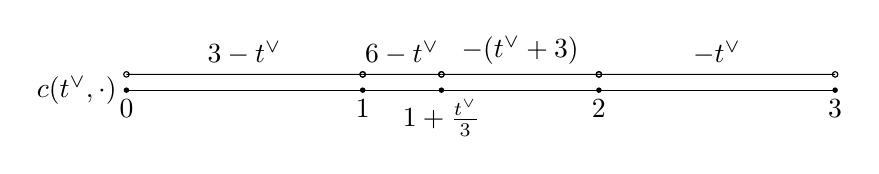
\begin{tikzpicture}[domain=0:9]
    
    \draw[-] (0,-1) node[left]{$c(t^\vee,\cdot)$} -- (9,-1);
    \fill (0,-1) circle (1pt) node[below] {$0$};
    \fill (3,-1) circle (1pt) node[below] {$1$};
    \fill (6,-1) circle (1pt) node[below] {$2$};
    \fill (9,-1) circle (1pt) node[below] {$3$};
    \draw (0,-0.8) circle[radius=1pt] to [edge label=$3-t^\vee$] (3,-0.8) circle[radius=1pt];
    \draw (3,-0.8) circle[radius=1pt] to [edge label=$6-t^\vee$] (4,-0.8) circle[radius=1pt];
    \draw (4,-0.8) circle[radius=1pt] to [edge label=$-(t^\vee+3)$] (6,-0.8) circle[radius=1pt];
    \draw (6,-0.8) circle[radius=1pt] to [edge label=$-t^\vee$] (9,-0.8) circle[radius=1pt];
    \fill (4,-1) circle (1pt) node[below] {$1+\frac{t^\vee}{3}$};
\end{tikzpicture}
\end{center}
Now, let $\ell \in \QQ_{>0}$ be such that $L^\ell_K$ is a line bundle. Then, $\ell = \frac{k}{3}$ for some positive integer $k$. If $m = \frac{a}{k}m_0+\frac{b}{k}m_1$ with $a,b\geq 0,a+b=k$, then $p(t^\vee) = m$ for $t^\vee = \frac{3b}{a+b}$. By hypothesis, we have $val_n(s^\ell_m) = \ell c(m,n)$, whence we see that the function $n\mapsto val_n(s^\ell_m)$ has the following slopes.
\begin{center}
    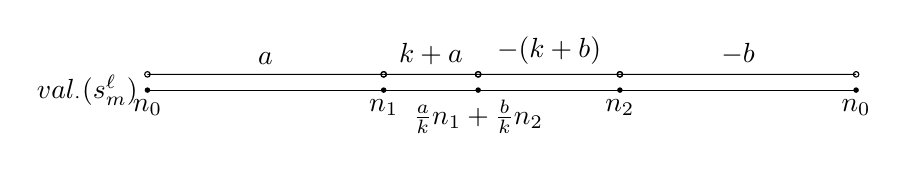
\begin{tikzpicture}[domain=0:9]
    
    \draw[-] (0,-1) node[left]{$val_\cdot(s^\ell_m)$} -- (9,-1);
    \fill (0,-1) circle (1pt) node[below] {$n_0$};
    \fill (3,-1) circle (1pt) node[below] {$n_1$};
    \fill (6,-1) circle (1pt) node[below] {$n_2$};
    \fill (9,-1) circle (1pt) node[below] {$n_0$};
    \draw (0,-0.8) circle[radius=1pt] to [edge label=$a$] (3,-0.8) circle[radius=1pt];
    \draw (3,-0.8) circle[radius=1pt] to [edge label=$k+a$] (4.2,-0.8) circle[radius=1pt];
    \draw (4.2,-0.8) circle[radius=1pt] to [edge label=$-(k+b)$] (6,-0.8) circle[radius=1pt];
    \draw (6,-0.8) circle[radius=1pt] to [edge label=$-b$] (9,-0.8) circle[radius=1pt];
    \fill (4.2,-1) circle (1pt) node[below] {$\frac{a}{k}n_1+\frac{b}{k}n_2$};
\end{tikzpicture}
\end{center}
Since our set-up is symmetric, similar statements hold when $m\in [m_1,m_2]$ or $m\in[m_2,m_0]$. It follows that if $n=(1-r)n_i+rn_{i+1}$ with $r \in [0,1]\setminus\{0,\frac{1}{k},\frac{2}{k},\dots,\frac{k-1}{k},1\}$, then each of the functions $n \mapsto val_n(s^\ell_m)$ is differentiable at $n$ and the collection of all their slopes at $n$ is precisely 
\[
\{0,\pm 1,\pm 2,\dots,\pm k, k+1,k+2,\dots, k+k-s, -(k+1),-(k+2),\dots,-(k+s-1)\}
\]
where $s$ is the positive integer such that $r\in (\frac{s-1}{k},\frac{s}{k})$. This set has cardinality $3k = |\partial \Delta_\ell|$, which shows that each member of the collection $s_m, m\in \partial\Delta_\ell$ has a distinct slope for $n = (1-r)n_i + rn_{i+1}$ as long as $r \in [0,1]\setminus\{0,\frac{1}{k},\frac{2}{k},\dots,\frac{k-1}{k},1\}$. Thus, for all but finitely many points $n\in \partial\Delta^\vee$, each section $s^\ell_m$ has a unique leading term in its Taylor expansion distinct from those of the other sections $s^\ell_{m^\prime}, m\neq m^\prime$. Therefore, the leading term in any $K$-linear combination must be given by taking the minimum over the leading terms of the summands since no cancellation is possible. Now since both sides of
\[
val_n\left(\sum_{m\in\partial\Delta_\ell}a_m s^\ell_m\right) = \min_{m\in\partial\Delta_\ell}\{val_t(a_m)+val_n(s^\ell_m) \ : \ a_m \neq 0 \}
\]
are continuous in $n$, the equality must still remain true for the remaining finitely many points.
\end{proof}

Thus, in order to establish the Theorem, it only remains to prove the first and the third statements. We shall do this inductively, using the explicit expression~\eqref{eq:Cost} for the cost function $c$.

Fix $\ell$ such that $L^\ell$ is a line bundle. We shall first define $s^\ell_m$ for $m=\frac{p}{p+q}m_0+\frac{q}{p+q}m_1 \in[m_0,m_1]$, for all values of $p,q =\ell \geq0$ as a polynomial expression in $x_0,x_1,x_2$ and $t$, homogeneous of degree $\ell$ in the $x_i$. Recall that $m=\frac{p}{p+q}m_0+\frac{q}{p+q}m_1 \in[m_0,m_1]$ corresponds to the $t^\vee = \frac{3q}{p+q}$, and from~\eqref{eq:Cost} we get that
\begin{equation}\label{eq:VanishingOrders}
    \frac{p+q}{3}c\left(\frac{3q}{p+q},r\right) = 
    \begin{cases}
        pr & \textrm{ if } r\in[0,1],\\
        \\
        (2p+q)r + C_1 & \textrm{ if } r\in [1,1+\frac{q}{p+q}],\\
        \\
        -(2q+p)r + C_2 & \textrm{ if } r\in[1+\frac{q}{p+q},2],\\
        \\
        -qr +C_3& \textrm{ if } r\in[2,3],
    \end{cases}
    \end{equation}
    for some constants $C_i$. 
We need to define sections $s^\ell_m$ whose Taylor expansions have vanishing orders prescribed by the various slopes of this function. We shall do this by induction on $p+q$, giving $s^\ell_m$ as a polynomial expression in $x_0,x_1,x_2, t$, homogeneous of degree $p+q$ in the $x_i$. To this end, write $S(p,q,x_0,x_1,x_2)$ for this expression for $s^\ell_m$. First of all, define the following base cases:
\[
S(1,0,x_0,x_1,x_2) = x_1, \quad S(0,1,x_0,x_1,x_2) = x_2, \quad S(1,1,x_0,x_1,x_2) = x_1x_2-tx_0^2.
\] 
This defines $S(p,q,x_0,x_1,x_2)$ whenever $p+q = 0,1,2$. Let us suppress notation for the moment and write $S(p,q)$ for $S(p,q,x_0,x_1,x_2)$. 
Define 
\begin{equation}\label{eq:BaseCases}
    S(p,0)=S(1,0)^p,\quad S(0,q)= S(0,1)^q, \quad S(p,p)=S(1,1)^p
\end{equation}
for all $p,q\geq 0$. Using the fact that the points $m_0$ and $m_1$ correspond, respectively, to $t^\vee=0$ and $t^\vee=3$, it is quite straightforward to verify, using~\eqref{eq:Cost}, that 
\[
val_n(S(p,0)) = \frac{p}{3}c(m_0,n), \quad val_n(S(0,q))=\frac{q}{3}c(m_1,n).
\]
The following Lemma shows that the analogous statement is true also for $S(p,p)$. 
\begin{lemma}\label{lemma:EqualityCase}
    Let $p\geq1$. Then, the Taylor expansion of $S(p,p)$ in $x=x_1/x_0,y=x_2/x_0$ is of the form 
    \[
    S(p,p) = x^py^p\left(\left(\frac{y^3}{1+y^3}\right)^p + \left(\frac{x^3}{1+x^3}\right)^p + x^3y^3H_{p,p}(x^3,y^3)\right)
    \]
where every  nonzero monomial term in the power series $x^3y^3H_{p,q}(x^3,y^3)$ is dominated by $x^{3p}+y^{3p}$. Moreover, for $n\in\partial\Delta^\vee$, we have 
\[
val_n(S(p,p))=\frac{2p}{3}c(\frac{1}{2}m_0+\frac{1}{2}m_1,n).
\]
\end{lemma}
Above and hereafter, we say that a power series $f(x,y)$ \emph{dominates} another power series $g(x,y)$ if $val_n(f)\leq val_n(g)$ for each $n\in[n_1,n_2]$. With this terminology, if $f_1$ dominates $g_1$ and $f_2$ dominates $g_2$, then $f_1\cdot f_2$ dominates $g_1\cdot g_2$, and if the coefficients of all monomial terms of $f_1$ and $f_2$ are positive, then $f_1+f_2$ dominates $g_1\pm g_2$. 
\begin{proof}[Proof Lemma~\ref{lemma:EqualityCase}]
Computing the Taylor expansion of $S(p,p)$ and re-arranging the infinite sums, we get
    \begin{align*}
        S(p,p)&=(x_1x_2-tx_0^2)^p \\
        &= \left(xy-\frac{xy}{1+x^3+y^3}\right)^p\\
        &=x^py^p\left(\frac{x^3+y^3}{1+x^3+y^3}\right)^p\\
        &=x^py^p(x^3+y^3)^p\left(\sum_{k=0}^\infty(-1)^k \binom{p-1+k}{k} (x^3+y^3)^k \right)\\
        &= x^py^p\left(x^{3p} \sum_{k=0}^\infty(-1)^k \binom{p-1+k}{k} x^{3k} + y^{3p}\sum_{k=0}^\infty(-1)^k \binom{p-1+k}{k} y^{3k} + x^3y^3 H_{p,p}(x^3,y^3)\right)\\
        &= x^py^p\left(\left(\frac{y^3}{1+y^3}\right)^p + \left(\frac{x^3}{1+x^3}\right)^p + x^3y^3H_{p,p}(x^3,y^3)\right),
    \end{align*}
    for some power series $H_{p,p}(x^3,y^3)$. (In the intermediate steps, we have used a well-known formula for the Taylor expansion of powers of the geometric series.) Now, every nonzero monomial term in $x^3y^3H_{p,p}(x^3,y^3)$ is of the form $\lambda x^{3\ell}y^{3s}$ with $\lambda \neq 0$ and $\ell,s\geq 1, \ell+s\geq 3p$. This is clearly dominated by $x^{3p}+y^{3p}$. Thus, $S(p,p)$ is dominated by $x^py^p(x^{3p}+y^{3p})$ and the coefficients of the terms $x^py^p\cdot x^{3p}, x^py^p\cdot y^{3p}$ in its Taylor expansion are equal to 1. 

     Comparing with \eqref{eq:VanishingOrders}, the above shows that functions $n\mapsto val_n(S(1,1))$ and $n\mapsto \frac{2p}{3}c(\frac{1}{2}m_0+\frac{1}{2}m_1,n)$ have the same slopes for $n\in[n_1,n_2]$. In order to establish that 
    \[
    val_n(S(1,1))=\frac{2p}{3}c(m,n)
    \]
    holds for all $n\in\partial\Delta^\vee$, we will show they also have the same slopes at all other points $n \in \partial\Delta^\vee$, and both functions are equal to $0$ at $n_0$. That $c(\frac{1}{2}m_0+\frac{1}{2}m_1,n_0)=0$ is readily verified from \eqref{eq:Cost}. Let $n\in[n_0,n_1]$. Then, the Taylor expansion of $S(p,p)$ in $\xi=x_0/x_2,\eta=x_1/x_0$ is given by 
    \[
    S(p,p)=\left(\eta-\frac{\xi^3\eta}{1+\xi^3+\eta^3}\right)^p=\eta^p\left(\frac{1+\eta^3}{1+\xi^3+\eta^3}\right)
    \]
    which is dominated by $\eta^p$ and the coefficient of $\eta^p$ in this Taylor expansion is equal to $1$. This shows that $val_{n_0}(S(1,1))=0$ and the two functions $n\mapsto val_n(S(1,1))$ and $n\mapsto \frac{2p}{3}c(\frac{1}{2}m_0+\frac{1}{2}m_1,n)$ have the same slopes for all $n\in[n_0,n_1]$. A similar argument shows they have the same slopes for $n\in[n_2,n_0]$.
\end{proof}

From now on, fix $a,b\geq 1$ and assume that  $S(p,q)$ has been defined for $p+q<a+b$ in such a way that 
\[
val_n(S(p,q)) = \frac{p+q}{3}c(\frac{p}{p+q}m_0+\frac{q}{p+q}m_1,n).
\]
In other words, its slopes as a piecewise affine function on $\partial\Delta^\vee$ are as follows.
\begin{center}
    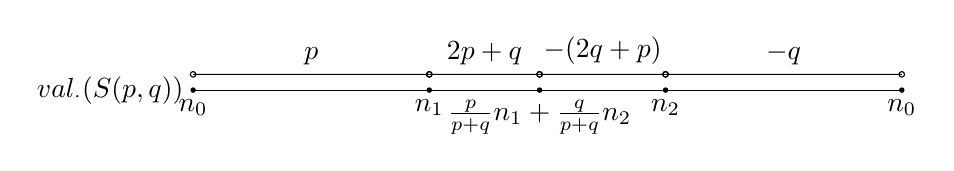
\begin{tikzpicture}[domain=0:9]
    
    \draw[-] (0,-1) node[left]{$val_\cdot(S(p,q))$} -- (9,-1);
    \fill (0,-1) circle (1pt) node[below] {$n_0$};
    \fill (3,-1) circle (1pt) node[below] {$n_1$};
    \fill (6,-1) circle (1pt) node[below] {$n_2$};
    \fill (9,-1) circle (1pt) node[below] {$n_0$};
    \draw (0,-0.8) circle[radius=1pt] to [edge label=$p$] (3,-0.8) circle[radius=1pt];
    \draw (3,-0.8) circle[radius=1pt] to [edge label=$2p+q$] (4.4,-0.8) circle[radius=1pt];
    \draw (4.4,-0.8) circle[radius=1pt] to [edge label=$-(2q+p)$] (6,-0.8) circle[radius=1pt];
    \draw (6,-0.8) circle[radius=1pt] to [edge label=$-q$] (9,-0.8) circle[radius=1pt];
    \fill (4.4,-1) circle (1pt) node[below] {$\frac{p}{p+q}n_1+\frac{q}{p+q}n_2$};
\end{tikzpicture}
\end{center}

This implies that, when $p,q\geq 1$, the Taylor expansion $S(p,q)$ in $x=x_1/x_0,y=x_2/x_0$ is of the form 
\[
S(p,q) = x^py^q(\lambda y^{3p}+\mu x^{3q}+ F(x) + G(y) + xy H(x,y))
\]
where $\lambda,\mu\neq 0$, $F(x) = O(x^{3q+3}), G(y)=O(y^{3p+3})$ and every nonzero monomial term in $xyH(x,y)$ is dominated by $x^{3q}+y^{3p}$ for every $n\in[n_1,n_2]$. For our purposes, we shall adopt a stronger inductive hypothesis. Namely, we shall assume moreover that whenever $p,q\geq 1$, the Taylor expansion of $S(p,q)$ in $x,y$ is of the form
\begin{equation}\label{eqn:CorrectTaylorSeries}
    S(p,q) = x^py^q\left(\left(\frac{y^3}{1+y^3}\right)^p + \left(\frac{x^3}{1+x^3}\right)^q + x^3y^3H_{p,q}(x^3,y^3)\right)
\end{equation}
where every (mixed) nonzero monomial term in $x^3y^3H_{p,q}(x^3,y^3)$ is dominated by $x^{3q}+y^{3p}$. Note that implicit in our inductive hypothesis is the assumption that $S(p,q)/x^py^q$ is a power series in $x^3$ and $y^3$. Note also that the base case $S(1,1)$ satisfies this stronger hypothesis by Lemma~\ref{lemma:EqualityCase}. 

Let $a,b\geq 0$ and assume, by induction, that $S(p,q)$ has been defined for all $p,q$ such that $p+q < a+b$ satisfying 
\[
val_n(S(p,q)) = \frac{p+q}{3}c\left(\frac{p}{p+q}m_0+\frac{q}{p+q}m_1,n\right)
\]
for all $n\in\partial\Delta^\vee$ and satisfying~\eqref{eqn:CorrectTaylorSeries} if $p,q\geq 1$. If $a=b$ or one of $a,b$ is zero, Lemma~\ref{} and the remarks preceding it show that we can define $S(a,b)$ by ~\eqref{eq:BaseCases}, so assume that $a,b\geq 1, a\neq b$. Define the section $R_0(a,b)\in H^0(X,L^{(a+b)/3})$ given by 
\[
R_0(a,b) = \begin{cases}
    x_1S(a-1,b)-t^2x_0S(a-2,b+1) & \textrm{ if } a>b\geq 1,\\
    \\
    x_2S(a,b-1)-t^2x_0S(a+1,b-2) & \textrm{ if } b > a\geq 1.
\end{cases}
\]
\begin{lemma}\label{lemma:R_0(a,b)}
    The Taylor expansion of $R_0(a,b)$ in $x,y$ is of the form
    \[
    R_0(a,b)=x^ay^b\left(\left(\frac{y^3}{1+y}\right)^{a}+\left(\frac{x^3}{1+x^3}\right)^{b}+x^3y^3G_{a,b}(x^3,y^3)\right)
    \]
    where $G_{a,b}(x^3,y^3)$ is some power series. Moreover, if $a>b\geq1$ (respectively, $b>a\geq 1$), then each nonzero monomial term in $x^3y^3G_{a,b}(x^3y^3)$ is dominated by $y^{3a-3}+x^{3b}$ (respectively, $y^{3a}+x^{3b-3}$).
\end{lemma}
\begin{rem}
    Note that we do not (and in fact cannot truthfully) make the stronger claim that the nonzero monomial terms in $x^3y^3G_{a,b}(x^3,y^3)$ are dominated by $y^{3a}+x^{3b}$.
\end{rem}
\begin{proof}[Proof of Lemma~\ref{lemma:R_0(a,b)}]
    Assume that $a>b\geq 1$. (The case whereby $b> a \geq 1$ is handled similarly by interchanging the roles of $x$ and $y$.) Then, by the inductive hypothesis~\eqref{eqn:CorrectTaylorSeries}, we have 
    \[
    S(a-1,b) = x^{a-1}y^b\left(\left(\frac{y^3}{1+y^3}\right)^{a-1} + \left(\frac{x^3}{1+x^3}\right)^{b} + x^3y^3H_{a-1,b}(x^3,y^3)\right)
    \]
    and 
    \[
    S(a-2,b+1) = x^{a-2}y^{b+1}\left(\left(\frac{y^3}{1+y^3}\right)^{a-2} + \left(\frac{x^3}{1+x^3}\right)^{b+1} + x^3y^3H_{a-2,b+1}(x^3,y^3)\right).
    \]
    Now observe that 
    \[
    t = \left(\frac{xy}{1+x^3+y^3}\right)=xy\left(\frac{x^3}{1+x^3}+\frac{1}{1+y^3}+x^3y^3F(x^3,y^3)\right) 
    \]
    for some power series $F(x^3,y^3)$. This in turn shows that 
    \[
    t^2=x^2y^2\left(\frac{1}{(1+y^3)^2}+x^3\tilde F(x^3,y^3)\right)
    \]
    for a power series $x^3\tilde F(x^3,y^3)$. Therefore we get
    \begin{align*}
    t^2x_0S(a-2,b+1) &=x^{a}y^{b+3}\left(\left(\frac{y^3}{1+y^3}\right)^{a-2} + \left(\frac{x^3}{1+x^3}\right)^{b+1} + x^3y^3H_{a-2,b+1}(x^3,y^3)\right)\left(\frac{1}{(1+y^3)^2}+x^3\tilde F(x^3,y^3)\right)\\
    &=x^{a}y^b\left(\frac{y^3}{(1+y^3)^2}\left(\frac{y^3}{1+y^3}\right)^{a-2}+x^3y^3G(x^3,y^3)\right) 
    \end{align*}
    for some power series $G(x^3,y^3)$. Thus, we conclude that 
    \begin{align*}
    R_0(a,b) &= x^{a}y^b\left(\left(\frac{y^3}{1+y^3}\right)^{a-1} +\left(\frac{x^3}{1+x^3}\right)^{b} -\frac{y^3}{(1+y^3)^2}\left(\frac{y^3}{1+y^3}\right)^{a-2}  + x^3y^3G_{a,b}(x^3,y^3)\right)\\
    &=x^ay^b\left(\left(\frac{y^3}{1+y}\right)^{a}+\left(\frac{x^3}{1+x^3}\right)^{b}+x^3y^3G_{a,b}(x^3,y^3)\right).
    \end{align*}
    for a power series $G_{a,b}(x^3,y^3)$. Now, by the inductive definition of $R_0(a,b)$, we see that each  nonzero monomial term in $R_0(a,b)$ is dominated by 
    \[x\cdot x^{a-1}y^b(y^{3a-3}+x^{3b})+x^2y^2\cdot x^{a-2}y^{b+1}(y^{3a-6}+x^{3b+3})
    \] 
    which itself is dominated by $x^ay^b(y^{3a-3}+x^{3b})$. This proves the Lemma.
\end{proof}
The above Lemma shows that $R_0(a,b)$ has the correct `pure' terms $x^ay^b(y^{3a}+x^{3b})$ but unfortunately, except for certain special cases, $R_0(a,b)$ will have several mixed terms that dominate these pure terms for some values of $n\in [n_1,n_2]$, and we still need to correct for these. Fortunately, there are only finitely many such terms, and it is easy to determine them explicitly. 
To this end, let us specialise to the case whereby $a>b\geq 1$. Then, by Lemma~\ref{lemma:R_0(a,b)}, $R_0(a,b)$ is dominated by $x^ay^b(y^{3a-3}+x^{3b})$, and every nonzero monomial term in $R_0(a,b)$ is of the form $\lambda x^ay^b\cdot x^{3
\ell}y^{3u}$. 

\begin{lemma}\label{lemma:BadTerms}
    Suppose $a>b\geq 1, \ell,u\geq1$ are positive integers. Then, the following are equivalent.
    \begin{enumerate}
        \item We have
        \[
        val_n(x^{3\ell}y^{3u}) \geq val_n(y^{3a-3}+ x^{3b}) \textrm{ for every } n\in\left[n_1,n_2\right]
        \]
        and
        \[
         val_n(x^{3\ell}y^{3u}) < val_n(y^{3a} + x^{3b}) \textrm{ for some } n\in\left[n_1,n_2\right].
         \]
         \item The pair $(\ell,u)$ belongs to $\Lambda_{a,b}$, where
         \[
         \Lambda_{a,b}=\left\{(m,s)\in\ZZ^2 \ : \ m>0,\ s>0, \   \frac{a}{b}m <a-s\leq \frac{a-1}{b}m+1\right\}.
         \]
    \end{enumerate}
\end{lemma}

\begin{proof}
    Writing $n\in[n_1,n_2]$ as $n=(1-r)n_1+rn_2$ for $r\in[0,1]$, we have 
    \[
        val_n(x^{3\ell}y^{3u}) \geq val_n(y^{3a-3}+ x^{3b}) \textrm{ for every } n\in\left[n_1,n_2\right]
    \]
        and
    \[
         val_n(x^{3\ell}y^{3u}) < val_n(y^{3a} + x^{3b}) \textrm{ for some } n\in\left[n_1,n_2\right]
    \]
    if and only if
    \[
    3ur+3\ell(1-r)\ge\min\{(3a-3)r,3b(1-r)\} \textrm{ for all } r\in[0,1],
    \]
    and 
    \[
    3ur+3\ell(1-r)<\min\{3ar,3b(1-r)\} \textrm { for some } r\in[0,1].
    \]
    Noting that $3ur+3\ell(1-r)$ depends affine linearly on $r$, and that the maximal values of $\min\{(3a-3)r,3b(1-r)\}$ and $\min\{3ar,3b(1-r)\}$ are respectively $3b(a-1)/(a+b-1)$ and $3ab/(a+b)$ and they are respectively achieved for $r=b/(a+b-1)$ and $r=b/(a+b)$, we see that this happens precisely when 
    \[
    3u\frac{b}{a+b}+3\ell\frac{a}{a+b}<\frac{3ab}{a+b} \quad \textrm{ and } \quad 3u\frac{b}{a+b-1}+3\ell\frac{a-1}{a+b-1}\geq \frac{3b(a-1)}{a+b-1},
    \]
    that is,
    \[
    a-\frac{a-1}{b}\ell - 1\leq u < a-\frac{a}{b}\ell.
    \]
    
\end{proof}
One way to restate the above Lemma is as follows: if a power series $F(x^3,y^3)$ is dominated by $y^{3a-3}+x^{3b}$ (and only involves terms of the form $x^{3p}y^{3q}$), and if the coefficient of $y^{3a-3}$ in $F(x^3,y^3)$ is zero, then it is in fact dominated by 
\[
y^{3a}+x^{3b}+\sum_{(m,s)\in\Lambda_{a,b}} x^{3m}y^{3s}.
\]
The set $\Lambda_{a,b}$ therefore corresponds to the set of potentially `bad terms' in $R_0(a,b)$ which will dominate $x^ay^b(y^{3a}+x^{3s})$ if they occur with nonzero coefficient. The next result essentially tells us that we can subtract off these terms in finitely many steps.
\begin{lemma}
    Suppose $a>b\geq1$. Then, the set $\Lambda_{a,b}$ is a finite set of cardinality
    \[
    k=\frac{b+\gcd(a-1,b)-\gcd(a,b)-1}{2}.
    \]
    In particular, $\Lambda_{a,b}=\varnothing$ if and only if $a$ is a multiple of $b$. Moreover, the maps $\Lambda_{a,b}\to \ZZ, (m,s)\mapsto m$ and $(m,s)\mapsto s-m$ are injective.
\end{lemma}
\begin{proof}
    Observe that $\Lambda_{a,b}$ is a subset of $D_{a,b}\cap \ZZ^2$ where $D_{a,b}$ is the convex set given by
    \[
    D_{a,b}=\left\{(m,s)\in\RR^2 \ : \ m\geq 0, \ s\geq 0, \ \frac{a}{b}m<a-s\leq \frac{a-1}{b}m+1\right\}.
    \]
    But now observe that $D_{a,b}$ is the convex hull of $(0,a-1)$, $(0,a)$ and $(b,0)$. This shows that $\Lambda_{a,b}$ is a finite set. By Pick's Theorem, the number of interior integral points in $D_{a,b}$ is given by
    \[
     \frac{b+1-\gcd(a,b)-\gcd(a-1,b)}{2},
    \]
    and since $\Lambda_{a,b}$ is the union of these interior integral points and the integral points on the interior of the edge joining $(0,a-1)$ and $(b,0)$, we get that $\Lambda_{a,b}$ has cardinality
    \[
    k=\frac{b+1-\gcd(a,b)-\gcd(a-1,b)}{2}+\gcd(a-1,b)-1 = \frac{b+\gcd(a-1,b)-\gcd(a,b)-1}{2}.
    \]
    If $a$ is a multiple of $b$, then $\gcd(a,b)=b, \gcd(a-1,b)=1$, and so $k=0$. Conversely, if $k=0$ then $b\geq \gcd(a,b) = b+\gcd(a-1,b) -1>b-1$, whence $\gcd(a,b)= b$ and so $a$ is a multiple of $b$.
    
    For the last claim, first assume $(m,s_1),(m,s_2)\in \Lambda_{a,b}$. Then we have 
    \[
    |s_1-s_2| < \left\vert\frac{a}{b}m-\frac{a-1}{b}m-1\right\vert=\left\vert1-\frac{m}{b}\right\vert < 1
    \]
    since $0<m<b$. This forces $s_1=s_2$. Next assume $(m,s),(m+e,s+e)\in\Lambda_{a,b}$ for some integer $e \geq 0$. If $e>0$ then we have 
    \[
    a-(s+e)>\frac{a}{b}(m+e)=\frac{a}{b}m+\frac{a}{b}e > \frac{a-1}{b}m+1 \geq a - s
    \]
    which is absurd. Hence, $e=0$.
\end{proof}

If $\Lambda_{a,b} = \varnothing$ (that is, $a$ is a multiple of $b$), then set $S(a,b) = R_0(a,b)$. Otherwise, write 
\[\Lambda_{a,b}=\{(m_1,s_1),(m_2,s_2),\dots,(m_k,s_k)\}
\] 
with $m_1<m_2<\dots<m_k$. Then, we have 
\[
a-s_i\leq\frac{a-1}{b}m_i+1<\frac{a}{b}m_i+\frac{a}{b}=\frac{a}{b}(m_i+1)\leq \frac{a}{b}m_{i+1}<a-s_{i+1}
\]
which shows that $s_1>s_2>\dots > s_k$. Set $d_i=s_i-m_i$. Then we have $0<d_i<a$ and $d_1>d_2>\dots > d_k$.  For $i=1,\dots, k$, define
\[
R_i(a,b)=
\begin{cases}
    R_{i-1}(a,b) - \lambda_it^{2a+5m_i-2s_i}x_0^{a-d_i}S(2d_i-a,a+b-d_i)& \textrm{ if } 3d_i > 2a,\\
    \\
    R_{i-1}(a,b) - \lambda_it^{a+3m_i}x_0^{2a-3d_i}x_2^{3d_i+b-a} & \textrm{ if } a-b\leq 3d_i \leq 2a,\\
    \\
    R_{i-1}(a,b)- \lambda_it^{b+3s_i}x_0^{2b+3d_i}x_1^{a-b-3d_i}& \textrm{ if } 3d_i < a-b,
    
\end{cases}
\]
where $\lambda_i$ is the coefficient of $x^ay^b\cdot x^{3m_i}y^{3s_i}$ in the Taylor expansion of $R_{i-1}(a,b)$ in $x$, $y$. Note that when $3d_i>2a$, $R_i(a,b)$ is well defined by the inductive hypothesis, since $(2d_i-a)+(a+b-d_i)=b+d_i<a+b$.
\begin{lemma}
    For each $i=0,1,\dots,k$, the Taylor expansion of $R_i(a,b)$ in $x,y$ is of the form
    \[
    R_i(a,b)=x^ay^b\left(\left(\frac{y^3}{1+y}\right)^{a}+\left(\frac{x^3}{1+x^3}\right)^{b}+x^3y^3G_{i,a,b}(x^3,y^3)\right)
    \]
    where every nonzero monomial term in $x^ay^b\cdot x^3y^3G_{i,a,b}(x^3,y^3)$ is dominated by 
    \[
    f_i=x^ay^b(y^{3a}+x^{3b}+\sum_{j>i}x^{3m_j}y^{3s_j}).
    \]
    In particular, every nonzero monomial term in the Taylor expansion of $R_k(a,b)$ is dominated by $x^ay^b(y^{3a}+x^{3b})$ and the coefficients of the $x^ay^b\cdot y^{3a}$ and $x^ay^b\cdot x^{3b}$ terms are both equal to $1$.

\end{lemma}
\begin{proof}
The statement is true for $i=0$ if we set $G_{0,a,b} = G_{a,b}$ given by Lemma~\ref{lemma:R_0(a,b)} above. Indeed, $x^3y^3G_{a,b}(x^3,y^3)$ is dominated by $y^{3a-3}+x^{3b}$ by Lemma~\ref{lemma:R_0(a,b)}. Then, the only monomial terms which dominate $y^{3a}+x^{3b}$ while being dominated by $y^{3a-3}+x^{3b}$ are precisely the ones occurring in $f_0$ by Lemma~\ref{lemma:BadTerms}. We can assume therefore $0<i\leq k$ and the conclusion holds for $R_{i-1}(a,b)$.

If $3d_i>2a$, then (by the inductive hypothesis) every nonzero monomial term in the Taylor expansion of $t^{2a+5m_i-2s_i}x_0^{a-d_i}S(2d_i-a,a+b-d_i)$ is a multiple of $x^ay^b\cdot x^{3m_i}y^{3a-3s_i+6m_i}$ and the coefficient of $x^ay^b\cdot x^{3m_i}y^{3s_i}$ is equal to $1$. (Note that $3a-3s_i+6m_i > 0$ as $0<s_i<a$.)

If $a-b\leq 3d_i\leq 2a$, then every nonzero monomial term in the Taylor expansion of $t^{a+3m_i}x_0^{2a-3d_i}x_2^{3d_i+b-a}$ is a multiple of $x^ay^b\cdot x^{3m_i}y^{3s_i}$ and the coefficient of $x^ay^b\cdot x^{3m_i}y^{3s_i}$ is equal to $1$.

If $3d_i<a-b$, then every nonzero monomial term in the Taylor expansion of $t^{b+3s_i}x_0^{2b+3d_i}x_1^{a-b-3d_i}$ is once again a multiple of $x^ay^b\cdot x^{3m_i}y^{3s_i}$ and the coefficient of $x^ay^b\cdot x^{3m_i}y^{3s_i}$ is again equal to $1$. 

This shows that in the Taylor expansion of $R_i(a,b)$ the `pure terms'
\[
x^ay^b \left(\left(\frac{y^3}{1+y^3}\right)^a + \left(\frac{x^3}{1+x^3}\right)^b\right)
\]
are the same as for $R_{i-1}(a,b)$, and hence the Taylor expansion of $R_i(a,b)$ is of the form 
\[
R_i(a,b)=x^ay^b\left(\left(\frac{y^3}{1+y}\right)^{a}+\left(\frac{x^3}{1+x^3}\right)^{b}+x^3y^3G_{i,a,b}(x^3,y^3)\right)
\]
for some power series $G_{i,a,b}(x^3,y^3)$. Moreover, it also shows that the coefficient of $x^ay^b\cdot x^{3m_i}y^{3s_i}$ in the Taylor expansion of $R_i(a,b)$ is zero. 

Now, by assumption $R_{i-1}(a,b)$ is dominated by
\[f_{i-1}=x^ay^b(y^{3a}+x^{3b} + \sum_{j\geq i}x^{3m_j}y^{3s_j})
\]
so the conclusion will follow once we establish that, in each of the three cases, the term being added to $R_{i-1}(a,b)$ to obtain $R_i(a,b)$ is also dominated by $f_{i-1}$, for this will imply (since $R_i(a,b)$ has no $x^ay^b(x^{3m_i}y^{3s_i})$ term by construction), that $R_i(a,b)$ is dominated by 
\[f_{i-1}-x^ay^b(x^{3m_i}y^{3s_i})= x^ay^b(y^{3a}+x^{3b} + \sum_{j> i}x^{3m_j}y^{3s_j}) = f_i.\]

If $3d_i>2a$, then by the inductive hypothesis $t^{2a+5m_i-2s_i}x_0^{a-d_i}S(2d_i-a,a+b-d_i)$ is dominated by 
\[
x^{a+3m_i}y^{b+3a-3d_i+3m_i}(y^{3(2d_i-a)}+x^{3(a+b-d_i)}) = x^{a}y^{b}(x^{3m_i}y^{3s_i}+x^{3b}\cdot x^{3(a-d_i+m_i)}\cdot y^{3a-3d_i+3m_i})
\]
which is dominated by $f_{i-1}$ since every one of its monomial terms is dominated by some monomial term of $f_{i-1}$. 

If $a-b\leq 3d_i \leq 2a$, then $t^{a+3m_i}x_0^{3a-3d_i}x_2^{3d_i+b-a}$ is dominated by $x^ay^b\cdot x^{3m_i}y^{3s_i}$ and therefore also by $f_{i-1}$. The case whereby $3d_i<a-b$ is identical.
\end{proof}

Finally, we can define $S(a,b)$ when $a>b\geq1$ and $a$ is not a multiple of $b$ by setting 
\[
S(a,b) = R_k(a,b).
\]

\begin{prop}
     For $n \in \partial\Delta^\vee$, we have 
    \[
    val_n(S(a,b)) = \frac{a+b}{3}c(n,\frac{a}{a+b}m_0+\frac{b}{a+b}m_1 ).
    \]
\end{prop}
\begin{proof}
    By construction the Taylor expansion of $S(a,b)$ in $x=x_1/x_0, y = x_2/x_0$ is dominated by $x^ay^b(y^{3a}+x^{3b})$ and these terms occur in $S(a,b)$ with coefficient equal to 1. Thus, the equality holds (by construction) for $n\in [n_1,n_2]$. Therefore, it only remains to establish the equality when $n\in [n_0,n_1]$ or $n\in[n_2,n_0]$. 
    
    Let $n\in[n_0,n_1]$. By the inductive hypothesis, the Taylor expansion of $S(p,q)$ in $\xi=x_0/x_2, \eta = x_1/x_2$ is dominated by $\eta^p$. From this, it follows that the Taylor expansion of $R_0(a,b)$ is dominated by $\eta^a+\eta^{a}\xi^3$ if $a>b \geq 1$ and therefore by $\eta^a$. Now suppose $R_{i-1}(a,b)$ is dominated by $\eta^a$. If $3d_i>2a$, then $R_i(a,b)$ is dominated by $\eta^a + \eta^{2a+5m_i-2s_i+2d_i-a}\xi^{a-d_i} = \eta^a(1+\eta^{3m_i}\xi^{a-d_i})$. If $a-b
    \leq 3d_i\leq 2a$, then $R_i(a,b)$ is dominated by $\eta^a+\eta^{a+3m_i}\xi^{2a-3d_i}$ and if $3d_i<a-b$ then $R_i(a,b)$ is dominated by $\eta^a+\eta^{b+3s_i+a-b-3d_i}\xi^{2b+3d_i}=\eta^{a}(1+\eta^{3m_i}\xi^{2b+3d_i})$. In all three cases, $R_i(a,b)$ is dominated by $\eta^a$. This shows that $S(a,b)$ is dominated by $\eta^a$. 
    
    Now, it is easy to see by the inductive hypothesis that $S(a,b) = x_1^ax_2^b+tS^\prime(a,b)$ for some section $S^\prime (a,b) \in H^0(X,\mathcal O(a+b))$, so the coefficient of $\eta^a$ in the Taylor expansion of $S(a,b)$ in $\xi,\eta$ is equal to $1$. This shows that for $n\in[n_0,n_1]$, we have 
    \[
    val_n(S(a,b))= val_n(\eta^a).
    \]
    This establishes the equality for $n\in[n_0,n_1]$. The case $n\in[n_2,n_0]$ is exactly the same, and we omit it to avoid repetition.
\end{proof}

This defines $S(a,b)$ whenever $a>b\geq 1$. We define $S(a,b)$ when $b>a\geq 1$ by interchanging the roles of $a$ and $b$ and $x_1$ and $x_2$ in the above construction. More precisely, recall the notation $S(a,b) = S(a,b,x_0,x_1,x_2)$ indicating how $S(a,b)$ depends on  $x_0,x_1,x_2$ explicitly. Then, if $b>a\geq 1$, we define
\[
S(a,b,x_0,x_1,x_2) = S(b,a,x_0,x_2,x_1).
\]
This process defines $s^{a+b}_m$ whenever $m\in[m_0,m_1]\cap(m_0+\frac{a+b}{3}\ZZ^2)$. By symmetry, we may therefore define
\[
s^{a+b}_m = \begin{cases}
    S(a,b,x_0,x_1,x_2) & \textrm{ if }\quad m=\frac{a}{a+b}m_0+\frac{b}{a+b}m_1,\\
    \\
    S(a,b,x_1,x_2,x_0) & \textrm{ if }\quad m=\frac{a}{a+b}m_1+\frac{b}{a+b}m_2,\\
    \\
    S(a,b,x_2,x_0,x_1) & \textrm{ if }\quad m=\frac{a}{a+b}m_2+\frac{b}{a+b}m_0.
\end{cases} 
\]
\begin{theorem}
    Let $\ell\in\QQ_{>0}$ be such that $L^\ell$ is a line bundle. For $m\in\partial\Delta\cap(m_0+\ell^{-1}\ZZ^2) = \partial\Delta_\ell$ denote by $\sigma_m \in H^0(X_K,L_K^\ell)$ the monomial section corresponding to $m$. Then, the following statements hold.
    \begin{enumerate}
        \item For every $m\in\partial\Delta_\ell$, we have $s_m= \sigma_m + ts_m^\prime$ for some $s_m^\prime \in H^0(X,L^\ell)$.
        \item When viewed as a basis for $H^0(X_K,L^\ell_K)$, the basis $s_m, m\in\partial\Delta_\ell$ is valuatively independent.
        \item For all $m\in\partial\Delta_\ell$, and $n\in\partial\Delta^\vee$ we have 
        \[
        \ell^{-1}val_n(s_m/\tau(n))=c(n,m).
        \]
    \end{enumerate}  
\end{theorem}
\begin{proof}
    The first and the third statements hold by construction. The second statement follows from the Proposition.
\end{proof}

It is worth noting that, although the basis $s_m$ itself is not uniquely determined by its being valuatively independent, the functions $n\mapsto val_n(s_m)$ are all uniquely determined. Indeed, suppose $\tilde s_m$ were another basis such that $\tilde s_m = \sigma_m + t\tilde s_m^\prime$ for some section $\tilde s^\prime_m\in H^0(X,L^\ell)$. Then, $s_m=(I+tB)\sigma_m$ and $\tilde s_m= (I+t\tilde B)\sigma_m$, whence we have that 
\[
\tilde s_m = (I+tB^\prime)s_m. 
\]
Writing $B^\prime = (b_{m m^\prime})$, we then have 
\[
\tilde s_m = (1+tb_{mm}) s_m + \sum_{m^\prime\neq m} b_{mm^\prime}s_{m^\prime}.
\]
Thus, we have 
\[
val_n(\tilde s_m) = \min\{val_t(1+tb_{mm})+val_n(s_m), \min_{m^\prime\neq m} \{1+val_t(b_{mm^\prime}) +val_n(s_{m^\prime})\}\} \leq val_n(s_m)
\]
since $val_t(1+tb_{mm})=0$. Similarly, $val_n(s_m)\leq val_n(\tilde s_m)$, so equality follows. 

\begin{thebibliography}{MMRZ22}

\bibitem[AH23]{AH} R. Andreasson, J. Hultgren. Solvability of Monge-Ampère equations and tropical affine structures on reflexive polytopes. \emph{arXiv:2303.05276}

\bibitem[HJMM22]{HJMM} J. Hultgren, M. Jonsson, E. Mazzon, N. McCleerey, Tropical and non-Archimedean Monge--Ampère equations for a class of Calabi--Yau hypersurfaces, \textit{Adv. Math.} \textbf{439} (2024), Article 109494.

\bibitem[HO19]{HO} 
J.~Hultgren and M.~\"Onnheim.
\newblock \emph{An optimal transport approach to Monge--Amp\`ere equations on compact Hessian manifolds}.
\newblock J. Geom. Anal. \textbf{29} (2019), 1953--1990.

\bibitem[Li22a]{LiFermat}
Y Li, Strominger--Yau--Zaslow conjecture for Calabi--Yau hypersurfaces in the Fermat family, \textit{Acta Math.} \textbf{229} (2022), 1--53.

\bibitem[Li23a]{LiNA}
\underline{\hspace{1.5cm}}, Metric SYZ conjecture and non-Archimedean geometry, \textit{Duke Math. J.} \textbf{172} (2023), no. 17, 3227--3255.

\bibitem[Li24b]{LiToric} \underline{\hspace{1.5cm}}, Metric SYZ conjecture for certain toric Fano hypersurfaces, \textit{Camb. J. Math.} \textbf{12} (2024), no. 1, 223--252.

\bibitem[Li25]{LiCanonicalBasis} \underline{\hspace{1.5cm}}, Degeneration of Calabi-Yau metrics and canonical basis. \emph{arXiv:2505.11087}

\bibitem[PS22]{PS} L. Pille-Schneider. Hybrid toric varieties and the non-archimedean SYZ fibration on Calabi--Yau hypersurfaces, \emph{arXiv:2210.05578}.

\end{thebibliography}




\end{document}

